\section{Теоретические сведения}

Если на концах нити машины Атвуда висят грузы одинаковой массы, то система находится в равновесии: движения грузов не происходит. Однако если между массами грузов существует разница (этого можно добиться, например, за счёт укладывания перегрузков на основные грузы), то они будут двигаться равноускоренно в противоположных вертикальных направлениях. Рассмотрим этот процесс детальнее с точки зрения динамики.

\begin{wrapfigure}{r}{0.25\textwidth}
    \centering
    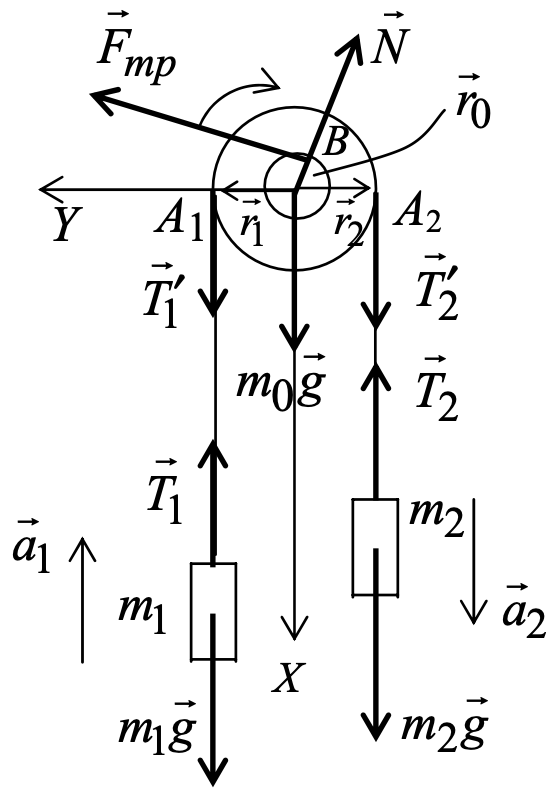
\includegraphics[width=0.25\textwidth]{pictures/PictureOne}
    \caption{Блок массой $m_0$ с грузами}\label{PictureOne}
\end{wrapfigure}
Направим ось абсцисс $Ox$ вертикально вниз, ось ординат $Oy$ --- горизонтально влево, а ось аппликат $Oz$ --- перпендикулярно плоскости рисунка от наблюдателя (рис.~\ref{PictureOne}). Таким образом мы получим правую систему координат. Пусть грузы имеют массы $m_1$ и $m_2$, и при этом $m_2>m_1$. Пренебрегая силами сопротивления воздуха, запишем уравнения движения грузов:
\begin{gather}
	m_1\vec a_1=m_1\vec g+\vec T_1, \\
	m_2\vec a_2=m_2\vec g+\vec T_2,
\end{gather}
где $\vec a_i$ --- ускорение груза массы $m_i$ ($i\in\{\;1,2\;\}$), $\vec g$ --- ускорение свободного падения, $\vec T_i$ --- сила натяжения нити, приложенная к грузу массы $m_i$. Будем считать, что нить нерастяжима, а значит,
\begin{equation}
	\vec a_1=-\vec a_2, \quad a_1=a_2=a.
\end{equation}
При этом ускорения грузов не имеют составляющих по координатным осям, кроме оси абсцисс. Их проекции на последнюю совпадают по модулю, но противоположны по знаку:
\begin{equation}
-a_{1x}=a_{2x}=a.
\end{equation}
Для проекций прочих величин выполняются следующие соотношения:
\begin{equation}
g_x=g,\quad T_{1x}=-T_1,\quad T_{2x}=-T_2.
\end{equation}

Исключим проскальзывание нити по блоку. По третьему закону Ньютона, $\vec F=-\vec N$, где $\vec F$ --- сила давления на ось блока, $\vec N$ --- сила реакции его оси. Значит,
\begin{equation}\label{EqSix}
F_\text{тр}=\mu N,
\end{equation}
где $F_\text{тр}$ --- равнодействующая сил трения, $\mu$ --- коэффициент трения между блоком и осью. Силы, действующие на блок, взаимно уравновешиваются, а значит,
\begin{equation}\label{EqSeven}
m_0\vec g+\vec T_1'+\vec T_2'+\vec N+\vec F_\text{тр}=0,
\end{equation}
где $\vec T_1'$ и $\vec T_2'$ --- силы натяжения нитей, приложенные в точках $A_1$ и $A_2$ соответсвенно. Из уравнений~\eqref{EqSix} и~\eqref{EqSeven} следует
\begin{equation}\label{EqEight}
F_\text{тр}=\frac{\mu}{\sqrt{1+\mu^2}}\left(T_1'+T_2'+m_0g\right)\approx\mu\left(T_1'+T_2'+m_0g\right),
\end{equation}
поскольку в нашем случае $\mu<0{,}1$. Силы натяжения нитей, а так же $\vec F_\text{тр}$ и $\vec N$ остаются неизменными в ходе опыта.

Уравнение моментов для блока имеет вид
\begin{equation}
J\vec\beta=\vec M_1+\vec M_2+\vec M_\text{тр},
\end{equation}
где $J$ --- момент инерции блока, $\vec\beta$ --- угловое ускорение блока, $\vec M_\text{тр}$ --- момент сил трения в его оси, $\vec M_1$ и $M_2$ --- моменты сил натяжения нитей $\vec T_1'$ и $\vec T_2'$. При этом
\begin{equation}
\vec M_1=\left[\vec r_1,\vec T_1'\right],\quad\vec M_2=\left[\vec r_2,\vec T_2'\right],
\end{equation}
где $\vec r_1$ и $\vec r_2$ --- составляющие радиус-векторов точек $A_1$ и $A_2$, перпендикулярные к оси вращения блока. Момент $\vec M_2$ направлен по оси аппликат, а $\vec M_1$ --- в противоположную сторону:
\begin{equation}
M_{1z}=-M_1=-rT_1',\quad M_{2z}=M_2=rT_2',
\end{equation}
где $r=r_1=r_2$ --- радиус блока.

Момент сил трения вычисляется по формуле
\begin{equation}
\vec M_\text{тр}=\left[\vec r_0,\vec F_\text{тр}\right]=\text{const},
\end{equation}
где $r_0$ --- перпендикулярная к оси вращения блока составляющая радиус-вектора точки $B$ приложения сил $\vec F_\text{тр}$ и $\vec N$. Поскольку угловое ускорение блока направлено по оси $Oz$, а момент сил трения --- в противоположную сторону, то
\begin{equation}
\beta_z=\beta,\quad M_{\text{тр}z}=-M_\text{тр}.
\end{equation}
Заметим также, что
\begin{equation}
J=\alpha m_0r^2,
\end{equation}
где $0<\alpha<1$.

Будем считать нить невесомой. Исходя из третьего закона Ньютона,
\[
\vec T_1'=-\vec T_1,\quad\vec T_2'=-\vec T_2.
\]
На основании записанных выше данных, получим систему
\begin{equation}\label{EqFifteen}
\left\{
\begin{array}{l}
	-m_1a=m_1g-T_1 \\
	m_2a=m_2g-T_2 \\
	\alpha m_0r^2\beta=r(T_2-T_1)-M_\text{тр}
\end{array}
\right.
.
\end{equation}
Учитывая соотношение
\begin{equation}\label{EqSixteen}
a=\beta r
\end{equation}
при решении системы~\eqref{EqFifteen}, придём к следующему:
\begin{equation}\label{EqSeventeen}
a=\cfrac{(m_2-m_1)g-\cfrac{M_\text{тр}}{r}}{m_1+m_2+\alpha m_0}=\text{const}.
\end{equation}
Если выполнены условия
\begin{gather}
m_1+m_2\gg\alpha m_0,\label{EqEighteen} \\
(m_2-m_1)rg\gg M_\text{тр},\label{EqNeinteen} 
\end{gather}
\begin{figure}[h]
	\begin{center}
		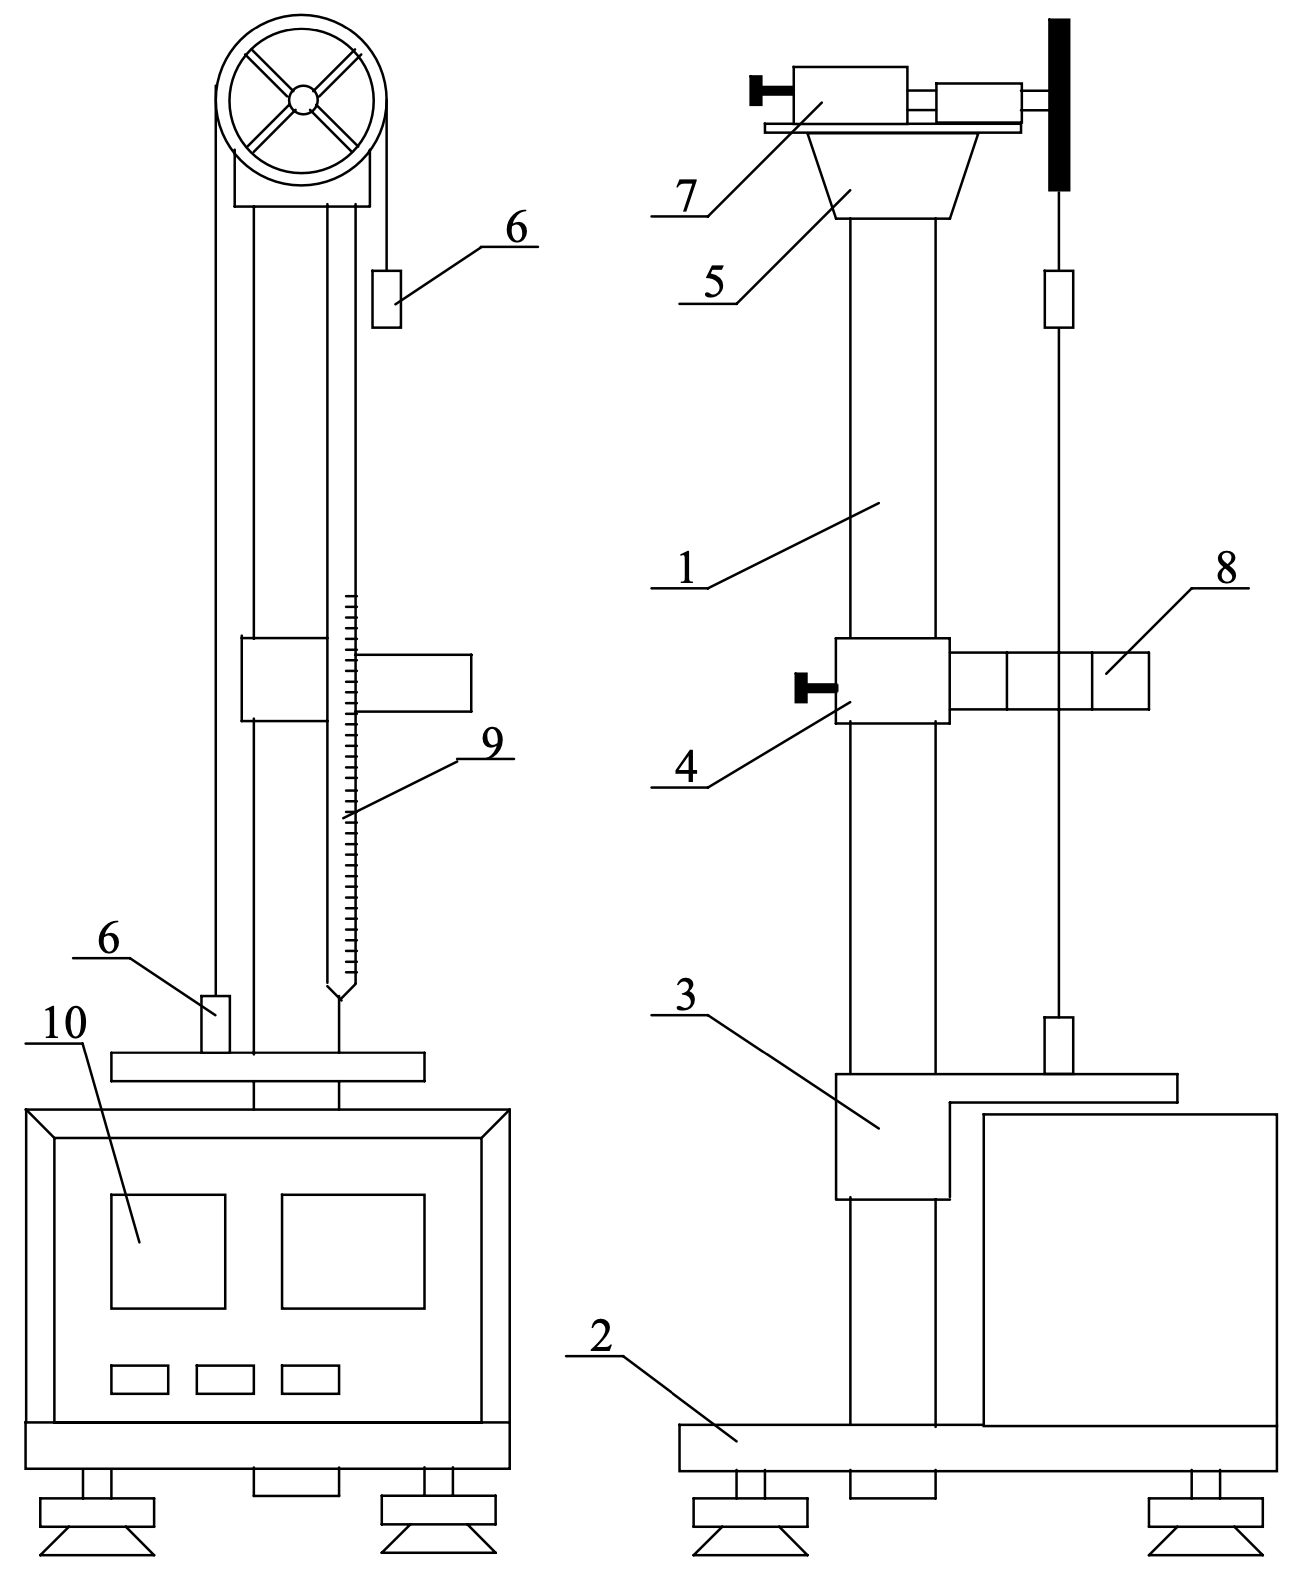
\includegraphics[width=0.6\textwidth]{pictures/PictureTwo}
		\caption{Машина Атвуда}\label{PicTwo}
	\end{center}
\end{figure}
то
\begin{equation}
a\approx\frac{(m_2-m_1)g}{m_1+m_2}.
\end{equation}
Последние допущения приводят к увеличению теоретического значения ускорения.

В том случае, если движение грузов начинается из состояния покоя, то путь $h$ пройденный каждым из грузов за время $t$, определяется формулой
\begin{equation}
h=\frac{at^2}{2}.
\end{equation}

Если на одном из грузов находится перегрузок массой $m_1'$, а на другом --- $m_2'>m_1'$, то
\begin{equation}
m_1=m+m_1',\quad m_2=m+m_2',
\end{equation}
где $m$ --- масса свободного от них груза. Тогда, с учётом названных выше приближений,
\begin{equation}
a=\frac{\left(m_2'-m_1'\right)g}{2m+m_1'+m_2'}.
\end{equation}
Если же перегрузки установлены так, что
\begin{equation}
m_1=m,\quad m_2=m+m_1'+m_2',
\end{equation}
то имеем
\begin{equation}
a'=\frac{\left(m_1'+m_2'\right)g}{2m+m_1'+m_2'}.
\end{equation}
В конечном счёте, получаем
\begin{equation}\label{EqTwentysix}
\frac{a}{a'}=\frac{m_2'-m_1'}{m_1'+m_2'}.
\end{equation}